\chapter{Segnali aperiodici nel dominio della frequenza}

\begin{figure}[h]
    \centering
    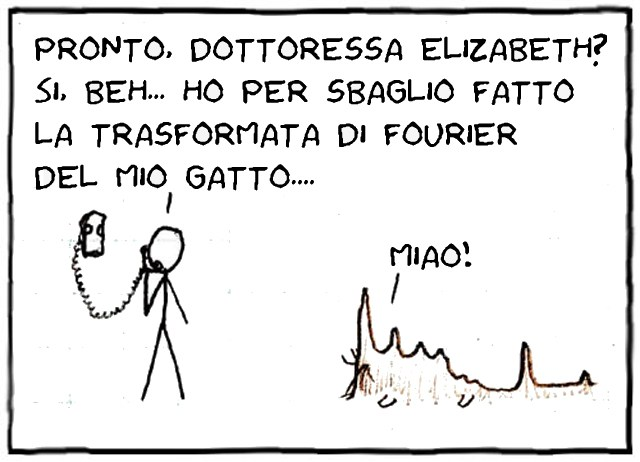
\includegraphics[scale = 3]{meme a caso.jpg}
\end{figure}  

\newpage 

\section{Trasformata di Fourier}

Dai segnali periodici del capitolo precedente, passiamo ora ai segnali aperiodici. \newline 

I segnali aperiodici possono essere visti come segnali periodici con T che tende ad infinito:  

{
    \Large 
    \begin{equation}
        T \rightarrow + \infty 
        \leftrightarrow 
        \omega_0 \rightarrow 0
    \end{equation}
}

Non possiamo definire uno sviluppo in serie di Fourier, bensì la nuova rappresentazione 
per un segnale aperiodico si chiamerà trasformata di Fourier definita come: 

{
    \Large 
    \begin{equation}
        S(\omega) = F[s(t)] = \int_{-\infty}^{+\infty} s(t) e^{-\jmath \omega t} dt 
    \end{equation}
}

L'anti-trasformata di Fourier, cioè l'inverso della trasformata di Fourier, è definito come: 

{
    \Large 
    \begin{equation}
        s(t) = F^{-1} [S(\omega)] = \frac{1}{2 \pi} \int_{-\infty}^{+\infty} S(\omega) e^{\jmath \omega t} d\omega
    \end{equation}
}

Quindi possiamo vedere lo stesso segnale come: 

{
    \Large
    \begin{equation}
        s(t) 
        \leftrightarrow 
        S(\omega)
    \end{equation}
}

Come lo sviluppo in serie di Fourier, possiamo definire lo spettro di ampiezza e di fase 
per una trasformata di Fourier: 

{
    \Large 
    \begin{equation}
        S(\omega) = \abs{S(\omega)} e^{\jmath \theta_s (\omega)}
    \end{equation}
}

A differenza della serie di Fourier, gli spettri non saranno a righe, bensì continui. \newline 

\newpage 

\section{Caratteristiche di un segnale Fourier trasformabile} 

Come nel caso dei segnali in serie di Fourier, 
non tutti i segnali possono essere Fourier trasformabili. \newline 

I segnali devono essere assolutamente integrabili: 

{
    \Large 
    \begin{equation}
        \int_{-\infty}^{+\infty} \abs{s(t)} dt < \infty
    \end{equation}
} 

I segnali che sono assolutamente integrabili vengono detti impulsivi. \newline 

Se il segnale s(t) è reale: 

{
    \Large
    \begin{equation}
        \begin{cases}
            \Re[S(-\omega)] = \Re[S(\omega)] \\ 
            \Im [S(-\omega)] = -\Im[S(\omega)]
        \end{cases}
        \leftrightarrow
        \begin{cases}
            \abs{S(-\omega)} = \abs{S(\omega)} \\ 
            \theta_s (-\omega) = - \theta_s (\omega)
        \end{cases}
    \end{equation}
}

dove: 
{
    \Large 
    \begin{equation}
        \Re[S(\omega)] = \int_{-\infty}^{+\infty} s(t) \cos(\omega t ) dt
    \end{equation}
}

{
    \Large 
    \begin{equation}
        \Im[S(\omega)] = \int_{-\infty}^{+\infty} - s(t) \sin(\omega t ) dt
    \end{equation}
}

Se s(t) è reale pari, la sua trasformata è reale pari:

{
    \Large 
    \begin{equation}
        \Re[S(\omega)] = \Re[S(-\omega)]
    \end{equation}
}

{
    \Large 
    \begin{equation}
        \Im[S(\omega)] = 0
    \end{equation}
}

Se s(t) è reale dispari, la sua trasformata è immaginaria dipari:

{
    \Large 
    \begin{equation}
        \Re[S(\omega)] = 0
    \end{equation}
}

{
    \Large 
    \begin{equation}
        \Im[S(\omega)] = -\Im[S(-\omega)] 
    \end{equation}
}


\newpage 

\section{Proprietà della trasformata di Fourier} 

Anche questo tipo di rappresentazione, ammette delle proprietà: \newline 

\textbf{Proprietà della traslazione temporale} 

{
    \Large
    \begin{equation}
        s^{'} (t) = s(t - \tau) 
        \leftrightarrow 
        S^{'} (\omega) = S(\omega) e^{-\jmath \omega \tau}
    \end{equation}
}

\textbf{Proprietà della traslazione in frequenza}

Considerando $\omega_1$ la frequenza traslata, possiamo dire che: 

{
    \Large 
    \begin{equation}
        s^{'} (t) = s(t) e^{\jmath \omega_1 t} 
        \leftrightarrow 
        S^{'} (\omega) = S(\omega -\omega_1)
    \end{equation}
}


\textbf{Proprietà di inversione dell'asse temporale}

{
    \Large 
    \begin{equation}
        s^{'} (t) = s (-t)
        \leftrightarrow 
        S^{'} (\omega) = S(\omega)
    \end{equation}
}

\textbf{Proprietà del coniugo}

{
    \Large
    \begin{equation}
        s^{'} (t) = s^{*} (t)
        \leftrightarrow 
        S^{'} = S^{*} (-\omega)
    \end{equation}
}

\textbf{Proprietà della derivazione}

{
    \Large
    \begin{equation}
        s^{'} (t) = \frac{d^{m} s(t)}{dt^{m}}
        \leftrightarrow
        S^{'} (\omega) = S(\omega) (\jmath \omega) ^{m}
    \end{equation}
}

\textbf{Proprietà dell'integrazione} 

Se il valore medio è nullo:

{
    \Large 
    \begin{equation} 
        S(\omega = 0) = \int_{- \infty}^{+ \infty} s(t) dt = 0
    \end{equation}
}

allora: 

{
    \Large 
    \begin{equation}
        S^{'} (t) = \int_{- \infty}^{t} s(t) dt 
        \leftrightarrow
        S^{'} (\omega) = \frac{S(\omega)}{\jmath \omega}
    \end{equation}
}

Grazie alla proprietà dei segnali impulsivi, quindi all'introduzione della Delta di Dirac, 
possiamo definire la trasformata di Fourier generalizzata anche per segnali con valore medio non nullo: 

{
    \Large 
    \begin{equation}
        s^{'} (t) = \int_{- \infty}^{t} s(t) dt 
        \leftrightarrow 
        S^{'} (\omega) = \frac{S(\omega)}{\jmath \omega} + \pi S(\omega = 0) \delta(\omega)
    \end{equation}
}

\textbf{Proprietà della moltiplicazione per t}

{
    \Large
    \begin{equation}
        s^{'} (t) = t ^{m} s(t) 
        \leftrightarrow
        S^{\omega} = \jmath ^{m} \frac{d^{m} S(\omega)}{d\omega ^{m}}
    \end{equation}
}

\textbf{Proprietà di dualità}

Dato un segnale s(t) la cui trasformata sia $S(\omega)$, la trasformazione di S(t) risulta 
$2\pi s(-\omega)$: 

{
    \Large 
    \begin{equation}
        s(t) \leftrightarrow S(\omega) 
        \text{  implica } 
        S(t) \leftrightarrow 2\pi s(-\omega)
    \end{equation}
}

Questa proprietà è molto importante perchè l'andamento del segnale di inizio del tempo alla 
rappresentazione in trasformata di Fourier è uguale all'andamento del segnale da trasformata 
di Fourier al segnale nel tempo sono uguali a meno di un fattore di $2 \pi$. \newline 

Quindi t e $\omega$ sono interscambiali. \newline 


\textbf{Proprietà di linearità} 

{
    \Large 
    \begin{equation}
        s^{'} (t) = A_1 s_1(t) + A_2 s_2(t) 
        \leftrightarrow 
        S^{'} (\omega) = A_1 s_1(\omega) + A_2 s_2(\omega)
    \end{equation}
} 

\textbf{Proprietà della convoluzione} 

{
    \Large 
    \begin{equation}
        \begin{split}
            c(t) 
            &= \int_{- \infty}^{+\infty} s_1(\tau) s_2(t-\tau) d\tau 
            \\
            &= s_1 (t) \otimes s_2 (t) \\
            &\updownarrow 
            \\ 
           C(\omega) &= S_1(\omega) S_2(\omega)    
        \end{split}
    \end{equation}
}

L'integrazione viene svolta su $\tau$ e t viene visto come parametro nella formula di integrazione. \newline 

\textbf{Proprietà del prodotto}

{
    \Large 
    \begin{equation}
        s^{'} (t) = s_1(t) s_2 (t) 
        \leftrightarrow 
        S^{'}(\omega) = \frac{1}{2 \pi} \int_{-\infty}^{\infty}S_1(\theta) S_2 (\omega - \theta) d\theta
    \end{equation}
}

L'integrazione viene svolta su $\theta$ e $\omega$ viene visto come parametro nella formula di integrazione. \newline 

A meno della costante $\frac{1}{2 \pi}$, questa proprietà si dimostra grazie alla proprietà di dualità. \newline 

\newpage 

\section{Altre caratteristiche sulla dualità tempo-frequenza} 

Di seguito verranno elencate alcune caratteristiche sulla dualità tempo-frequenza. \newline 

{
    \begin{itemize}
        \item Un segnale s(t) che è limitato nel tempo, ha spettro illimitato sull'asse delle pulsazioni 
        \item Un segnale con spettro delle pulsazioni limitato, ha un'evoluzione temporale illimitata in t. \\ 
        (Questo si dimostra grazie alla proprietà di dualità tempo-frequenza spiegato nella sezione precedente) 
        \item Possiamo definire $B_\omega$ la larghezza significativa di un segnale, cioè l'intervallo di pulsazioni in cui il modulo di $S(\omega)$ assume valori non trascurabili, maggiori di una soglia minima prefissata: \\ 
        quanto maggiore risulta $B_\omega$, s(t) varierà più rapidamente. 
        \item Possiamo definire $D_t$ la durata significativa come l'intervallo di tempo in cui il segnale assume valori non trascurabili e definiamo Q come parametro di qualità. \\
        In formule: 
        {
            \Large 
            \begin{equation}
                B_\omega D_t \geq Q
            \end{equation}
        } 
        Generalmente: 
        {
            \Large 
            \begin{equation}
                Q = 2\pi
            \end{equation}
        } 
        
    \end{itemize}
}


\newpage 

\section{Teorema del cambiamento di scala} 

Un teorema che è importante sulla dualità tempo-frequenza è il seguente. \newline 


Consideriamo il segnale: 

{
    \Large 
    \begin{equation}
        y(t) = s(\alpha t)
    \end{equation}
}

Se consideriamo $S(\omega)$ la trasformata di Fourier di s(t), e $\alpha$ un parametro. \newline 

Al cambiare di $\alpha$, ci saranno degli effetti diversi sullo spettro di $S(\omega)$ : 

\begin{itemize}
    \item $\abs{\alpha} > 1 \rightarrow $ compressione della scala dei tempi 
    \item  $\abs{\alpha} < 1 \rightarrow $ dilatazione della scala dei tempi 
    \item $\alpha < 0 \rightarrow $ inversione della scala dei tempi 
\end{itemize}

Facendo la trasformata di Fourier di y(t), avremo che: 
{
    \Large 
    \begin{equation}
        y(t) = s(\alpha t) 
        \leftrightarrow 
        Y(\omega) = \frac{1}{\abs{\alpha}} S(\frac{\omega}{\alpha})
    \end{equation}
} 

Si nota che una dilatazione dell'asse dei tempi comporta una compressione dell'asse delle pulsazioni e viceversa. \newline 

\newpage 

\section{Teorema della modulazione} 

Consideriamo il segnale originale s(t) e consideriamo il nuovo segnale $s^{'} (t)$ e la sua trasformata di Fourier come: 

{
    \Large 
    \begin{equation}
        \begin{split}
            s^{'} (t) &= s(t)\cos(\omega_0 t) \\ 
            &\updownarrow \\
            S^{'} (\omega) &= \frac{1}{2} [S(\omega - \omega_0) + S(\omega + \omega_0)]    
        \end{split}
    \end{equation}
}

\subsection{Dimostrazione del teorema della modulazione} 

Utilizzando la formula di Eulero e l'argomento $\omega_0 t$: 

{
    \Large 
    \begin{equation}
        e^{\jmath \omega_0 t} = \cos(\omega_0 t) + \jmath \sin(\omega_0 t) = \jmath(-1)^{\omega_0 t}
    \end{equation}
}

Possiamo riscrivere: 

{
    \Large 
    \begin{equation}
        s^{'} (t) = s(t)\cos(\omega_0 t)
        \leftrightarrow 
        s^{'} (t) = s(t) \frac{e^{\jmath \omega_0 t} + e^{-\jmath \omega_0 t}}{2}
    \end{equation}
} 

Di qui, applicando le proprietà di linearità e di traslazione in frequenza, si ottiene: 

{
    \Large 
    \begin{equation}
        \begin{split}
            S^{'} (\omega) 
        &= 
        \frac{S (\omega - \omega_0) + S (\omega + \omega_0)}{2}
        \\ 
        &= 
        \frac{1}{2}
        [S (\omega - \omega_0) + S (\omega + \omega_0)]
        \end{split}
    \end{equation}
}

\newpage 

\subsection{Considerazioni sul teorema della modulazione} 

Dal teorema della modulazione, notiamo che se la trasformata di Fourier del segnale s(t) si espande 
nella banda $[- \omega_B, +\omega_B]$, lo stesso segnale si troverà centrato a destra in $\omega_0$ con banda 
$[\omega_0 - \omega_B, \omega_0 + \omega_B]$, lo stesso accade a sinistra dello spettro. \newline 

Il segnale sarà lo stesso di quello originario centrato in $- \omega_0$ e $\omega_0$ moltiplicato per $\frac{1}{2}$. \newline 

La figura seguente, spiega il teorema dal punto di vista grafico: 

\begin{figure}[h]
    \centering
    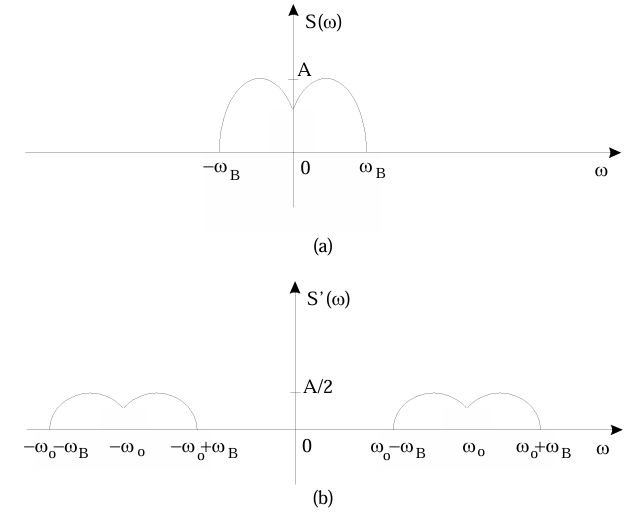
\includegraphics[scale = 1]{Teorema della modulazione visto graficamente.PNG}
\end{figure}  

La figura in alto viene definita come il segnale in banda base, cioè la banda in cui è s(t);  
mentre $S^{'} (\omega)$ viene definita come il segnale in banda traslata. \newline 

La porzione di spettro in cui $\abs{\omega} > \omega_0$  viene definita come banda laterale superiore, 
mentre la porzione di spettro per $\abs{\omega} < \omega_0$ prende la banda laterale inferiore. \newline 

Se il segnale s(t) è reale, allora le due sottobande godono di simmetria e lo spettro complessivo è simmetrico rispetto all'origine. \newline 

\newpage 
